\documentclass[conference]{IEEEtran}
\IEEEoverridecommandlockouts
% The preceding line is only needed to identify funding in the first footnote. If that is unneeded, please comment it out.
\usepackage{cite}
\usepackage{amsmath,amssymb,amsfonts}
\usepackage{algorithmic}
\usepackage{graphicx}
\usepackage{textcomp}
\usepackage{xcolor}
\usepackage{url}
\usepackage{hyperref} 
\usepackage{amsmath}

\def\BibTeX{{\rm B\kern-.05em{\sc i\kern-.025em b}\kern-.08em
    T\kern-.1667em\lower.7ex\hbox{E}\kern-.125emX}}
\begin{document}

\title{Sincronização de semáforos baseado em NTP\\}

\author{\IEEEauthorblockN{1\textsuperscript{st} André de Azevedo Barata}
\IEEEauthorblockA{
up201907705@up.pt}
\and
\IEEEauthorblockN{2\textsuperscript{nd} Diogo Vilela}
\IEEEauthorblockA{
up201907804@up.pt}

}

\maketitle

\begin{abstract}

\end{abstract}


\section{Introdução}


    Este trabalho apresenta um caso prático de sincronização de relógios usando o protocolo Network Time Protocol (NTP). O problema apresentado consiste em sincronizar as transições de estado de 4 semáforos de uma interseção sem que haja trocas de informações entre os eles. Deste modo, Todos os semáforos irão utilizar um relógio abstrato, escravizado de acordo com um servidor NTP, para inferir o seu estado (Verde, Vermelho).
    
    Por exemplo, considerando a figura \ref{fig:diagramaEstrada}, quando os semáforos da via horizontal (1 e 3) estão verdes, os via vertical (2 e 4) estão vermelhos. Ora, caso esta alteração de estado ocorra de $t$ em $t$ segundos, cada semáforo deve tomar essa decisão autonomamente de acordo com o seu relógio.
    Os quatro relógios apresentam características diferentes, pelo que $t$ segundo no semáforo 1 pode representar $t + \delta$ segundos no relógio 2, pelo que a transição no 2 seria tomada $\delta$ segundos mais tarde. Normalmente, $\delta$ é um valor muito pequeno, pelo que quando considerando uma só transição este valor é irrelevante. Contudo, esta discrepância acumula com o tempo e após duas transições já é de $2 \time \delta$, o que pode até levar ao caso de os dois semáforos estarem verdes ao mesmo tempo quando $N \times \delta = t$, em que $N$ é o número de transições ocorridas.
    A solução o problema é sincronizar os relógios do semáforos. Este processo não irá colocar $\delta$ a zero, mas sim mantê-lo com um valor baixo o suficiente para que seja irrelevante. Para tal. Cada semáforo irá atualizar periodicamente o "rate" e "offset" dos seus relógios com um servidor NTP, garantindo que $\delta$ não acumula infinitamente.  
    
    \begin{figure}[h]
        \centering
        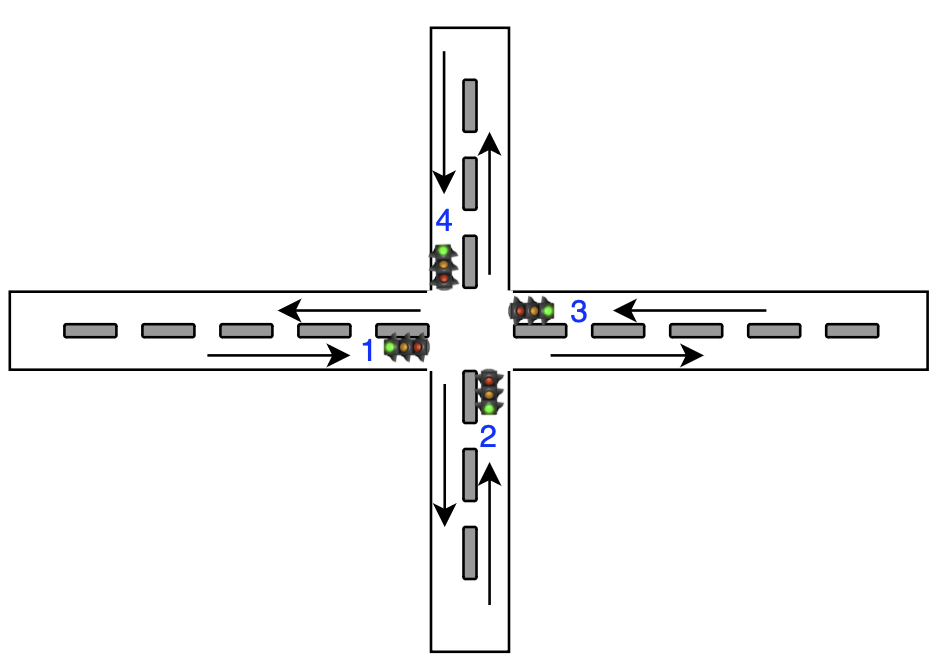
\includegraphics[width=0.8\linewidth]{figures/diagramaEstrada.png}
        \caption{Intresseção de uma estrada}
        \label{fig:diagramaEstrada}
    \end{figure}
\section{Protocolo NTP}
\label{sec:NTP}

O Network Time Protocol é um protocolo de sincronização
de relógios que sincroniza os relógios de um sistema distribuído 
através de redes com comutação de pacotes e de latência variável 
com uma precisão na ordem dos milissegundos. Este protocolo
foi primordialmente concebido para ter uma alta exatidão 
e fiabilidade \cite{b2}.

Para uma típica operação do protocolo NTP,
o cliente questiona um ou mais servidores NTP, de modo a 
receber o tempo atualizado. Após a receção dos dados do servidor, 
o cliente calcula o offset do seu relógio relativamente ao servidor, o delay da rede e o rate. Para tal, é necessário q ele saiba os timestamps da mensagem enviada por ele ao servidor e da consequente resposta do servidor,
para tal figura \ref{fig:diagramaNTP} contextualiza o protocolo de melhor
forma. Os timestamps que são necessário são então o tempo a que
a mensagem foi enviada pelo cliente, t0, e quando foi recebida pelo
servidor, t1, tal como quando a mensagem de resposta foi enviada
pelo servidor, t2, e finalmente recebida pelo cliente, t3.

    \begin{figure}[h]
        \centering
        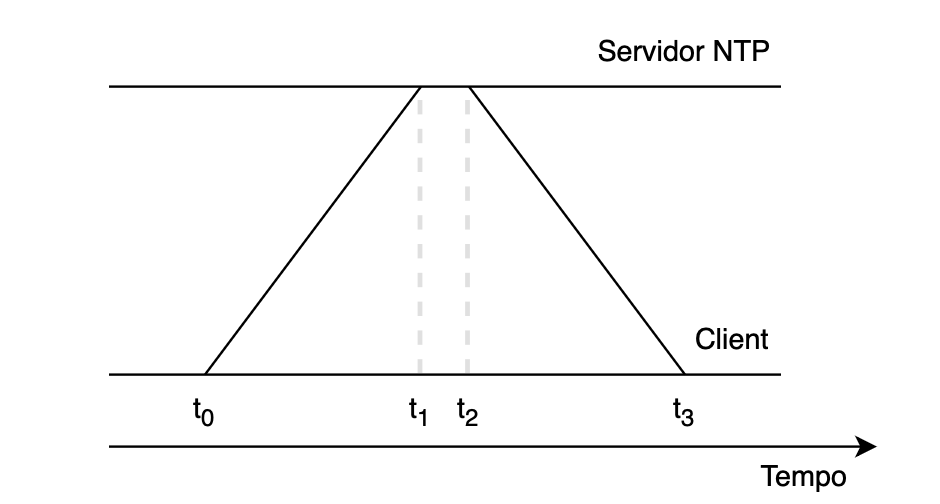
\includegraphics[width=0.8\linewidth]{figures/diagramaNTP.png}
        \caption{Ordem de eventos do protocolo NTP}
        \label{fig:diagramaNTP}
    \end{figure}

Com estes 4 tempos é então possível calcular quer o valor do offset quer o valor 
do delay da rede. O offset, $\theta$, vai corresponder 
à diferença entre o relógio do cliente e do servidor, sendo o valor dado pela equação \ref{eq:offset}. 


\begin{equation} \label{eq:offset}
\theta = \frac{\left( (t_{\text{1}} - t_{\text{0}}) + (t_{\text{2}} - t_{\text{3}}) \right)}{2} 
\end{equation}

O delay da rede, $\delta$, corresponde por sua vez ao tempo
que um pacote demora a ir do cliente ao servidor e vice-versa, sendo
o valor dado pela equação \ref{eq:delay}.


\begin{equation} \label{eq:delay}
\delta = (t_{\text{3}} - t_{\text{0}}) - (t_{\text{2}} - t_{\text{1}})
\end{equation}

Para além disso também pode ser calculado o rate, que serve
para compensar o desvio do relógio do cliente quando comparado com o do servidor.
Para tal, para o sistema criado no âmbito do projeto definiu-se a função do
rate de acordo com a equação \ref{eq:rate}. Na equação apresentada,
o valor $t_{\text{3}}'$ e $t_{\text{1}}'$ correspondem aos timestamps 
mais recentes, enquanto t1 e t3 correspondem aos timestamps da mensagem anterior à
atual. Assim, o rate vai sendo modificado com base nos timestamps
das duas últimas iterações entre cliente-servidor.


\begin{equation} \label{eq:rate}
\text{{rate}} =\left| \frac{{t_{\text{1}}' - t_{\text{1}} - \delta + \delta '}}{{t_{\text{3}}' - t_{\text{3}}}} \right|
\end{equation}


Por fim, a equação \ref{eq:corrected_time} foi concebida, de modo a corrigir
o tempo do relógio do cliente, sendo a variável \text{{elapsed\_time}} o tempo
que entre $t_{\text{3}}$ e o tempo em que a correção do tempo foi efetuada.


\begin{equation} \label{eq:corrected_time}
\text{{corrected\_time}} = t_{\text{3}} + \text{{elapsed\_time}} \cdot \text{{rate}} + \theta
\end{equation}



\section{Arquitetura do Sistema}

    Na interseção descrita na figura \ref{fig:diagramaEstrada} existem 4 semáforos, pelo que, idealmente, cada um seria representado por uma raspberrypi. Contudo, devido ao facto de apenas existirem duas raspberrypis disponíveis, os semáforos 1 e 3 são representados pela mesma raspberrypi e os semáforos 2 e 4 por outra, sendo que é considerado que quando os semáforos 1 e 3 têm sempre o mesmo e os semáforos 2 e 4 também. Assim, quando a raspberrypi A está no estado VERDE é permitido o transito horizontal e quando a raspberrypi B está VERDE é permitido o trânsito vertical. As raspberrypis nunca apresentam o mesmo estado em simultâneo. 

    O sistema foi desenhado de acordo com a figura \ref{fig:diagramaSistema}. Ambas as raspberrypis foram conectadas à rede Wi-Fi do portátil que por sua vez comunica com o servidor NTP \url{pool.ntp.org}. As cada raspberrypi representa um cliente que envia para o portátil os pedidos NTP de acordo com a secção \ref{sec:NTP} que por sua vez são reencaminhados para o servidor. A resposta faz o caminho oposto.
    O estado da cada raspberrypi é enviado para o portátil cada vez que existe uma transição. Este processo serve apenas para monitorização e está representado na figura como monitor. Este regista o tempo local de chegada da mudança de estado de cada estado e avalia a diferença de tempo entre a chegada do estado de cada raspberrypi. Por exemplo, quando A fica VERMELHO B deve ficar VERDE, o monitor avalia o desfasamento desta duas ações (que deve ser o menor possível).

    O protocolo empregue para a comunicação é o "Transmission Control Protocol" - TCP. Se o servidor NTP não responder à solicitação, é acionado um "timeout", e o sistema tenta restabelecer a ligação. Esta funcionalidade é crucial, uma vez que o servidor tem uma disponibilidade muito baixa, mas um tempo médio de reparação reduzido, permitindo assim uma rápida recuperação da ligação. Isso resulta em correções não periódicas, mas essa irregularidade não afeta significativamente a sincronização do sistema já que o sistema esforça-se para restabelecer a ligação o mais rapidamente possível. Para além disso, o facto do servidor responder em $t$ ou $t + 1$ não tem grande influência no ajuste, já que os relógios das raspberrypis continua a utilizar parâmetros antigos para a correção e não é esperado que estes se alterem subitamente.


    \begin{figure}[h]
        \centering
        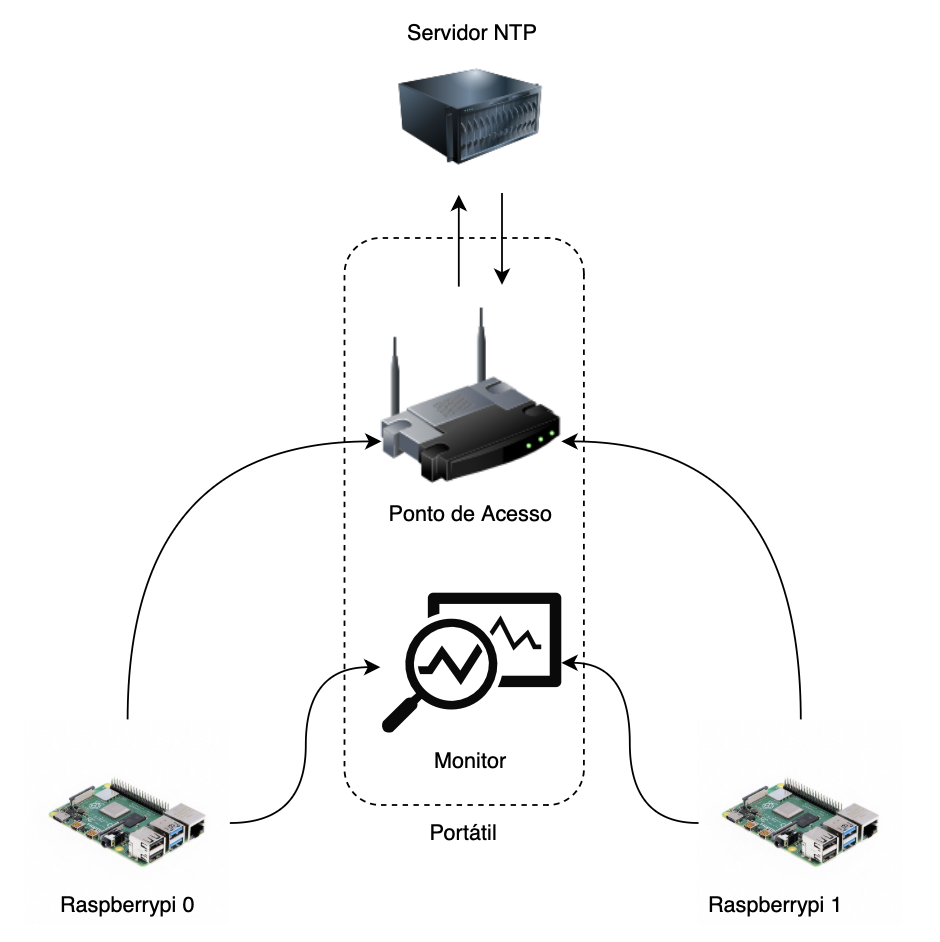
\includegraphics[width=0.8\linewidth]{figures/diagramaSistema.png}
        \caption{Diagrama da arquitetura do sistema \cite{b1}}
        \label{fig:diagramaSistema}
    \end{figure}


    
\section{Implementação} \label{sec:implementação}
    Durante esta secção, irá ser descrito o algoritmo de sincronização e posteriormente a sua implementação em Python. Para além disso, é feita a distinção entre três relógios:
    
    \begin{itemize}
        \item \textbf{Relógio monotónico}:  Relógio intrínseco do hardware. Nunca é corrigido e conta o tempo a partir do qual o sistema operativo foi iniciado.
        \item \textbf{Relógio NTP}: Relógio do servidor NTP e assumido como correto. Este relógio escraviza o sistema.
        \item \textbf{Relógio abstrato}: Relógio implementado em software em cima do sistema operativo. É o relógio monotónico corrigido em "rate" e "offset" de acordo com a secção \ref{sec:NTP}.
    \end{itemize}

    Posto isto, as raspberrypis têm dois relógios: monotónico e abstrato, sendo que este último é utilizado para tomar as decisões de mudança de estado. O monitor apenas utiliza o seu relógio monotónico para marcar os "timestamps" das mudanças de estado de A e B. O servidor NTP responde aos pedido com os "timestamps" do relógio NTP. 

\subsection{Algoritmo}
    O programa está dividido em dois processos distintos que ocorrem em paralelo: Correção do relógio e Atualizado do Estado. Ambos os algoritmos estão expressos em pseudo-código nas figuras \ref{fig:pseudoCodigoRelogio} e \ref{fig:pseudoCodigoEstado}, respetivamente.
    
    

    \begin{figure}[h]
        \centering
        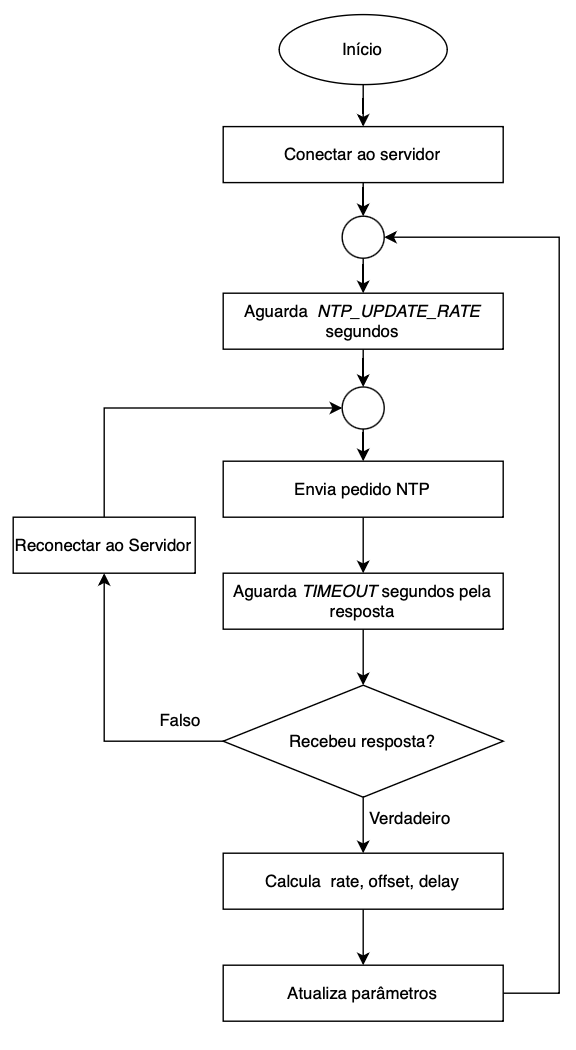
\includegraphics[width=0.6\linewidth]{figures/pseudoCodigoRelogio.png}
        \caption{Pseudo-código relativo à correção do relógio abstrato}
        \label{fig:pseudoCodigoRelogio}
    \end{figure}

    De referir que, o relógio abstrato é o relógio corrigido segundo os parâmetros obtido pelo último pedido NTP (offset, rate e delay), segundo as equações da secção \ref{sec:NTP}. A consulta do relógio abstrato consiste em calcular o tempo que passou desde da última correção NTP de acordo com o relógio monotónico, multiplicar esse tempo pelo rate, somar ao último timestamp desde a atualização e adicionar o offset, equação \ref{eq:corrected_time}.


    
    \begin{figure}[h]
        \centering
        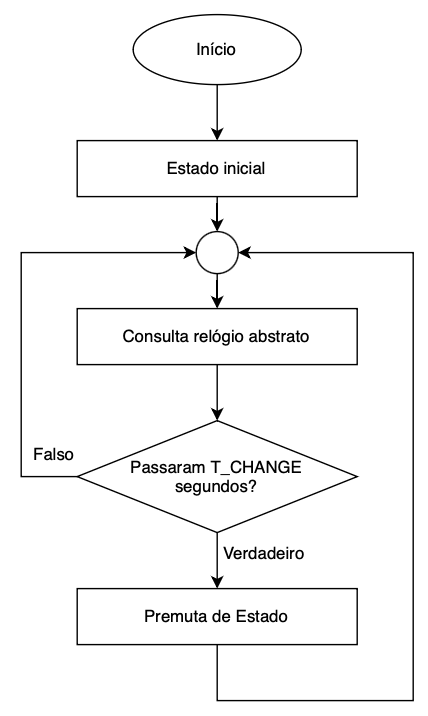
\includegraphics[width=0.6\linewidth]{figures/pseudoCodigoEstado.png}
        \caption{Pseudo-código relativo à atualização do estado}
        \label{fig:pseudoCodigoEstado}
    \end{figure}


\subsection{Implementação em Python}

\textcolor{red}{\textbf{Breve menção ao código, threads e class e referência ao git}
\section{Resultados} \label{sec:resultados}

\textcolor{red}{\textbf{Experiências em table: \\
    - Correção offset e rate\\
    - Correção só offset\\
    - Sem correcção\\
Resultados: \\
    - Erro nas slots \\
    - min, max, variação do rate, delay, offset}}
\input{inputTex/6_Conclusão}








\begin{thebibliography}{00}
\bibitem{b1} Digi-Key Electronics, https://www.digikey.pt/pt/products/detail/raspberry-pi/SC0194-9/10258781

\bibitem{b2} D.L. Mills. Internet time synchronization: the network time protocol. IEEE Transactions on Communications, 39(10):1482–1493, 1991.



\end{thebibliography}


\end{document}
